\section{Durchf\"{u}hrung}

Die Myonen, die gemessen werden sollen, entstehen größtenteils aus Pionzerfällen in der oberen Atmosphäre. Aufgrund ihrer relativistischen Energie erreichen sie den Erdboden. Durch Wechselwirkung mit Materie geben sie einen Teil ihrer kinetischen Energie ab. Bei Durchgang durch einen Szintillator in einem Edelstahltank regt die abgegebene Energie das Szintillatormaterial an, sodass bei der Rückkehr in den Grundzustand Photonen im kurzwelligen sichtbaren bis UV-Bereich emittiert werden. Diese Photonen werden mit zwei Sekundärelektronenvervielfachern (SEV) detektiert, die an den Enden des Tanks angebracht sind. Niederenergetische Myonen können innerhalb des Detektionsvolumen in ein Elektron zerfallen, welches ebenfalls durch einen Lichtblitz ein Signal auslöst. Der zeitliche Abstand zwischen dem Myon- und dem Elektronsignal ist dann die Lebensdauer des Myons im Tank.

Um nicht den zeitlichen Abstand verschiedener Myonen zu messen, sondern die Lebensdauer zerfallender Myonen, wird eine elektronische Stoppuhr verwendet. Nur wenn das Stoppsignal innerhalb der Suchzeit $T_\text{S}$ auf das Startsignal folgt, wird die Zeitdifferenz als Messwert für die Lebensdauer verwendet. Dies wird durch eine monostabile Kippstufe realisiert. Durch einen Startpuls wird für die Zeit $T_\text{S}$ ein Signal auf ein AND-Gatter gelegt; wenn in dieser Zeit ein weiterer Puls eintrifft, wird dies als Stoppuls interpretiert und die Zeitfifferenz dazwischen gemessen, andernfalls geht die Apperatur in den Grundzustand zurück und das nächste eintreffende Myon fungiert wieder als Startpuls. Der zeitliche Abstand zwischen Start- und Stoppuls wird mit einem Zeit-Amplituden-Konverter (TAC) in einen Spannungspuls umgewandelt, dessen Höhe linear mit der Dauer zusammenhängt. Die Höhe des Pulses wiederum wird mit einem Vielkanalanalysator ausgewertet. Der gesamte Messaufbau ist schematisch in \autoref{aufbau} dargestellt. Dieses Messverfahren gelingt, da die Abklingdauer des organischen Szintillators mit $\SI{10}{\nano\second}$ kleiner und der zeitliche Abstand verschiedener Myonen größer ist, als die mittlere Lebensdauer, die gemessen werden soll.
\begin{figure}
  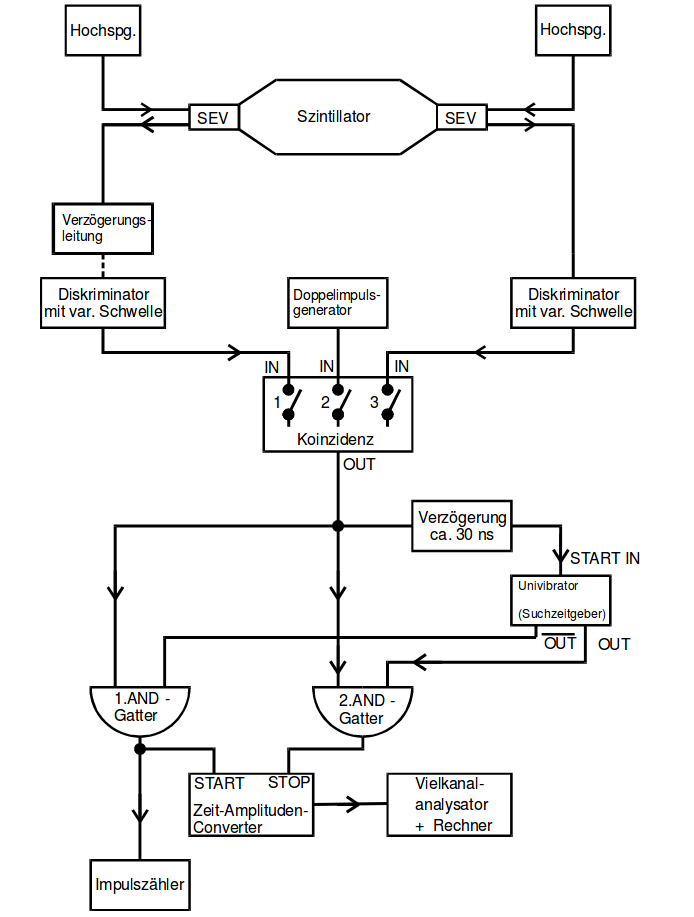
\includegraphics[width=\textwidth]{img/aufbau.png}
  \caption{Schematischer Aufbau der Messapparatur \cite{FP}}
  \label{aufbau}
\end{figure}

Der Diskriminator in \autoref{aufbau} dient dazu, Dunkelpulse zu filtern. Diese Dunkelpulse werden durch thermische Bewegung von Elektronen ausgelöst und besitzen in der Regel eine geringere Amplitude als Photonenpulse. Um keine echten Pulse zu verlieren, wird die Schwelle, bei der Pulse durchgelassen werden, nicht zu hoch eingestellt und als weiterer Filter eine Koinzidenz verwendet; nur wenn ein Signal von beiden SEVs eintrifft, wird es als Myonsignal akzeptiert.

Zur Einstellung der richtigen Diskriminatorschwelle wird zunächst ein Zählwerk angeschlossen und beide SEVs werden so eingeregelt, dass in beiden Kanälen jeweils eine Rate von 20 bis 40 pro Sekunde gemessen wird. Daraufhin wird die Koinzidenz eingestellt, indem eine Verzögerung so lange variiert wird bis ein Minimum in der Zählrate eintritt. Der TAC wird mit Hilfe eines Doppelpulsgenerators kalibriert; die Pulse werden mit einer Frequenz von $\SI{1}{\kilo\hertz}$ erzeugt und die Linearität zwischen dem Abstand der Pulse und der Amplitude der resultierenden Spannnung gezeigt. Die eigentliche Messung wird über mindestens 24 Stunden durchgeführt, um eine ausreichende Statistik zu erhalten, außerdem wird zum Ende der Messung notiert, wie viele Startpulse ohne Stoppulse und wie viele Startpulse mit Stoppulsen aufgetreten sind

\FloatBarrier
